\documentclass{beamer}
\usetheme{Singapore}
\usepackage{changepage}

%\usepackage{pstricks,pst-node,pst-tree}
\usepackage{amssymb,latexsym,dirtree}
\usepackage{tikz}
\usepackage{graphicx}
\usepackage{fancyvrb}
\usepackage{hyperref}
\usepackage{fancybox}
\usepackage[listings]{tcolorbox}

\definecolor{codegreen}{rgb}{0,0.6,0}
\definecolor{codegray}{rgb}{0.5,0.5,0.5}
\definecolor{codepurple}{rgb}{0.58,0,0.82}
\definecolor{backcolour}{rgb}{0.95,0.95,0.92}

\lstdefinestyle{mystyle}{
    language=Python,
    backgroundcolor=\color{backcolour},   
    commentstyle=\color{codegreen},
    keywordstyle=\color{magenta},
    numberstyle=\tiny\color{codegray},
    stringstyle=\color{codepurple},
    basicstyle=\ttfamily\normalsize,
    breakatwhitespace=false,         
    breaklines=true,                 
    captionpos=b,                    
    keepspaces=true,                 
    numbers=left,                    
    numbersep=5pt,                  
    showspaces=false,                
    showstringspaces=false,
    showtabs=false,                  
    tabsize=2,
    escapechar=|,
    frame=single
}

\lstset{style=mystyle}


\newcommand{\lst}[1]{\lstinline{#1}}

\newcommand{\lsting}[1]{\begin{lstlisting}[basicstyle=#1]}
\newcommand{\lstend}{\end{lstlisting}}

\newcommand{\bi}{\begin{itemize}}
\newcommand{\li}{\item}
\newcommand{\ei}{\end{itemize}}
\newcommand{\Show}[1]{
\begin{center}
\shadowbox{\begin{minipage}{0.8\textwidth}
          #1
          \end{minipage}}
\end{center}
}
\newcommand{\arrow}{\ensuremath{\rightarrow}}

\newcommand{\uparr}{\ensuremath{\uparrow}}


\newcommand{\fig}[2]{\centerline{\includegraphics[width=#1\textwidth]{#2}}}

\newcommand{\bfr}[1]{\begin{frame}[fragile]\frametitle{{ #1 }}}
\newcommand{\efr}{\end{frame}}

\newcommand{\cola}{\begin{columns}\begin{column}{0.6\textwidth}}
\newcommand{\colb}{\end{column}\begin{column}{0.4\textwidth}}
\newcommand{\colc}{\end{column}\end{columns}}


\title{\url{https://intro2r.com/} Chapter 3}
\author{CSCI 297b, Spring 2023}

\begin{document}

\begin{frame}
\maketitle
\end{frame}

\bfr{R basic data types}
\begin{description}
\li[Numeric] data are numbers that contain a decimal.


\li[Integers] are whole numbers.

\li[Logical data] take on the value of either TRUE or FALSE. 
There's also another special type of logical called NA to represent missing values.

\li[Character] data are used to represent string values. You can think of character strings as something like a word (or multiple words). A special type of character string is a factor, which is a string but with additional attributes (like levels or an order). We’ll cover factors later.
\end{description}
\end{frame}


\bfr{R basic data types}
\lsting{\small}
num <- 2.2
class(num)
## [1] "numeric"

char <- "hello"
class(char)
## [1] "character"

logi <- TRUE
class(logi)
## [1] "logical"
\end{lstlisting}
\end{frame}


\bfr{R basic data types}
\lsting{\small}
is.numeric(num)
## [1] TRUE

is.character(num)
## [1] FALSE

is.character(char)
## [1] TRUE

is.logical(logi)
## [1] TRUE
\end{lstlisting}
\end{frame}



\bfr{R type conversion}
\lsting{\small}
# coerce numeric to character
class(num)
## [1] "numeric"
num_char <-  as.character(num)
num_char
## [1] "2.2"
class(num_char)
## [1] "character"

# coerce character to numeric!
class(char)
## [1] "character"
char_num <- as.numeric(char)
## Warning: NAs introduced by coercion
\end{lstlisting}
\end{frame}

\bfr{Scalars and Vectors}

\cola
\bi
\li A vector with a single element is called a scalar.
\li Vectors can contain any single type.
\li You can't mix types in a vector.
\li NA can mix with any type.
\ei
\colb
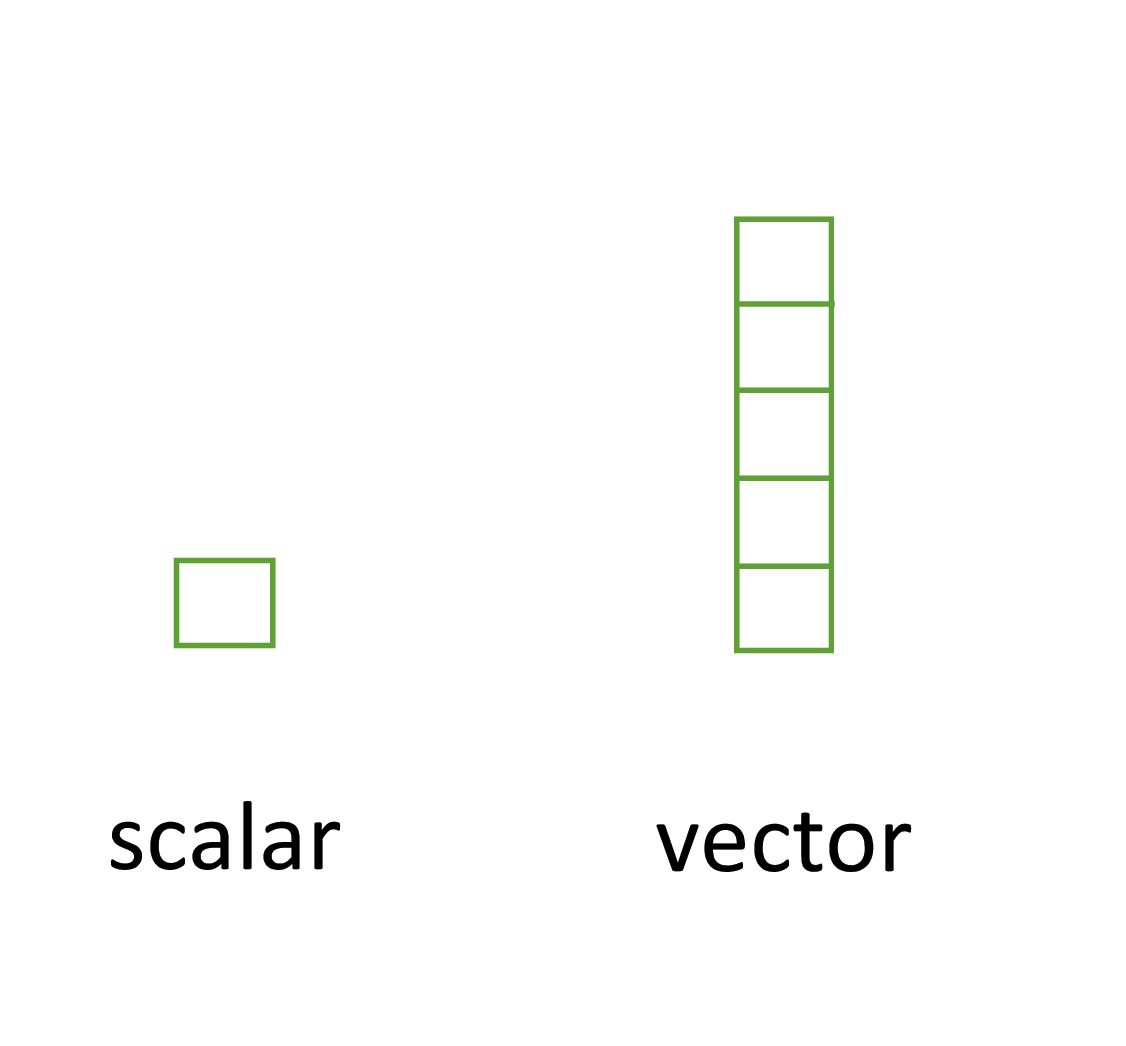
\includegraphics[width=\textwidth]{scal_vec}
\colc
\end{frame}



\bfr{Matrices and arrays}

\cola
\bi
\li A matrix is a vector with additional attributes called {\em dimensions}.
\li Arrays are multidimensional matrices.
\li Matrices and arrays can contain only a single type.
\li They may also contain NAs.
\ei
\colb
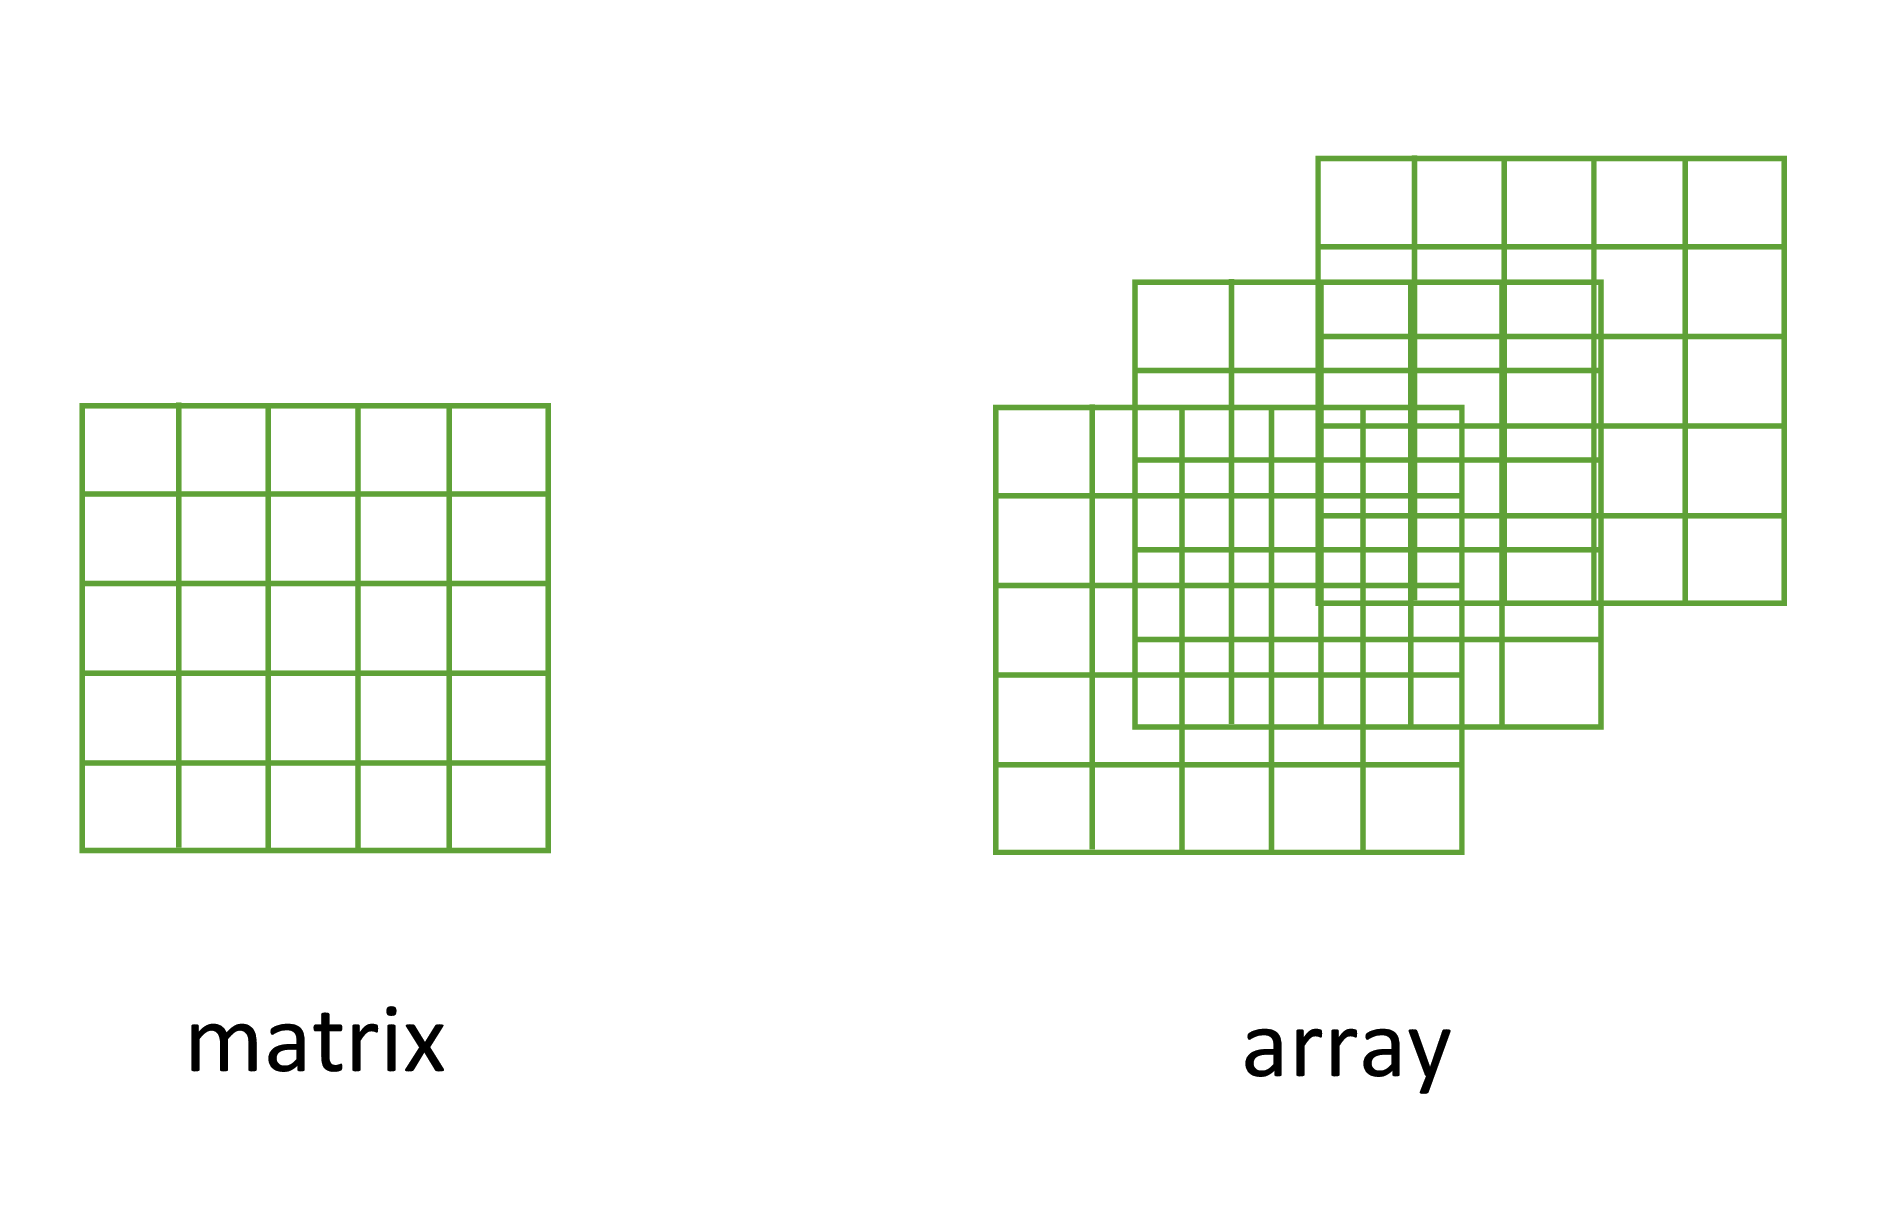
\includegraphics[width=\textwidth]{mat_array}
\colc
\end{frame}

\bfr{Creating matrices and arrays}
\lsting{\scriptsize}
my_mat <- matrix(1:16, nrow = 4, byrow = TRUE)
my_mat
##      [,1] [,2] [,3] [,4]
## [1,]    1    2    3    4
## [2,]    5    6    7    8
## [3,]    9   10   11   12
## [4,]   13   14   15   16

my_array <- array(1:16, dim = c(2, 4, 2))
my_array
## , , 1
## 
##      [,1] [,2] [,3] [,4]
## [1,]    1    3    5    7
## [2,]    2    4    6    8
## 
## , , 2
## 
##      [,1] [,2] [,3] [,4]
## [1,]    9   11   13   15
## [2,]   10   12   14   16
\end{lstlisting}
\end{frame}


\bfr{Optional row and column names}
\lsting{\scriptsize}
rownames(my_mat) <- c("A", "B", "C", "D")
colnames(my_mat) <- c("a", "b", "c", "d")
my_mat
##    a  b  c  d
## A  1  2  3  4
## B  5  6  7  8
## C  9 10 11 12
## D 13 14 15 16
\end{lstlisting}
\end{frame}


\bfr{Transpose a matrix}
\lsting{\scriptsize}
my_mat_t <- t(my_mat)
my_mat_t
##   A B  C  D
## a 1 5  9 13
## b 2 6 10 14
## c 3 7 11 15
## d 4 8 12 16
\end{lstlisting}
\end{frame}

\bfr{Diagonal elements}
\lsting{\scriptsize}
my_mat_diag <- diag(my_mat)
my_mat_diag
## [1]  1  6 11 16
\end{lstlisting}
\end{frame}

\bfr{Matrix arithmetic}
\lsting{\scriptsize}
mat.1 <- matrix(c(2, 0, 1, 1), nrow = 2)   
                 # notice that the matrix has been filled 
                 # column-wise by default
mat.1                         
##      [,1] [,2]
## [1,]    2    1
## [2,]    0    1

mat.2 <- matrix(c(1, 1, 0, 2), nrow = 2)
mat.2
##      [,1] [,2]
## [1,]    1    0
## [2,]    1    2

mat.1 + mat.2           # matrix addition
##      [,1] [,2]
## [1,]    3    1
## [2,]    1    3
mat.1 * mat.2           # element by element products
##      [,1] [,2]
## [1,]    2    0
## [2,]    0    2
\end{lstlisting}
\end{frame}

\bfr{Matrix multiplication }
\lsting{\scriptsize}
mat.1 <- matrix(c(2, 0, 1, 1), nrow = 2)  
mat.1                         
##      [,1] [,2]
## [1,]    2    1
## [2,]    0    1

mat.2 <- matrix(c(1, 1, 0, 2), nrow = 2)
mat.2
##      [,1] [,2]
## [1,]    1    0
## [2,]    1    2


mat.1 %*% mat.2         # matrix multiplication
##      [,1] [,2]
## [1,]    3    2
## [2,]    1    2
\end{lstlisting}
\end{frame}

\bfr{Lists}
\bi
\li Notice the double bracket [[ ]] for list items.
\ei
\lsting{\scriptsize}
list_1 <- list(c("black", "yellow", "orange"),
               c(TRUE, TRUE, FALSE, TRUE, FALSE, FALSE),
               matrix(1:6, nrow = 3))
list_1
## [[1]]
## [1] "black"  "yellow" "orange"
## 
## [[2]]
## [1]  TRUE  TRUE FALSE  TRUE FALSE FALSE
## 
## [[3]]
##      [,1] [,2]
## [1,]    1    4
## [2,]    2    5
## [3,]    3    6
\end{lstlisting}
\end{frame}

\bfr{List elements can be named}
\lsting{\scriptsize}
list_2 <- list(colours = c("black", "yellow", "orange"), 
               evaluation = c(TRUE, TRUE ,FALSE, 
                              TRUE, FALSE, FALSE), 
               time = matrix(1:6, nrow = 3))
list_2
## $colours
## [1] "black"  "yellow" "orange"
## 
## $evaluation
## [1]  TRUE  TRUE FALSE  TRUE FALSE FALSE
## 
## $time
##      [,1] [,2]
## [1,]    1    4
## [2,]    2    5
## [3,]    3    6
\end{lstlisting}
\end{frame}

\bfr{List elements can be renamed using \lst{names}}
\lsting{\scriptsize}
names(list_1) <- c("colours", "evaluation", "time")
list_1
## $colours
## [1] "black"  "yellow" "orange"
## 
## $evaluation
## [1]  TRUE  TRUE FALSE  TRUE FALSE FALSE
## 
## $time
##      [,1] [,2]
## [1,]    1    4
## [2,]    2    5
## [3,]    3    6
\end{lstlisting}
\end{frame}

\bfr{Data frames}
{\scriptsize
\begin{tabular}{llrrrrrr}
treat&	nitrogen&	block&	height&	weight&	leafarea&	shootarea&	flowers\\\hline
tip&	medium&	1&	7.5&	7.62&	11.7&	31.9&	1\\
tip&	medium&	1&	10.7&	12.14&	14.1&	46.0&	10\\
tip&	medium&	1&	11.2&	12.76&	7.1&	66.7&	10\\
tip&	medium&	1&	10.4&	8.78&	11.9&	20.3&	1\\
tip&	medium&	1&	10.4&	13.58&	14.5&	26.9&	4\\
tip&	medium&	1&	9.8&	10.08&	12.2&	72.7&	9\\
notip&	low&	2&	3.7&	8.10&	10.5&	60.5&	6\\
notip&	low&	2&	3.2&	7.45&	14.1&	38.1&	4\\
notip&	low&	2&	3.9&	9.19&	12.4&	52.6&	9\\
notip&	low&	2&	3.3&	8.92&	11.6&	55.2&	6\\
notip&	low&	2&	5.5&	8.44&	13.5&	77.6&	9\\
notip&	low&	2&	4.4&	10.60&	16.2&	63.3&	6\\
\end{tabular}
}
\bi
\li Most used data structure for real world data.
\li Each row contains an individual {\bf observation}.
\li Each column contains a measured {\bf variable}.
\li Each column is a vector of a single type.
\li Columns can be different types.
\ei
\end{frame}


\bfr{Data frames}
{\scriptsize
\begin{tabular}{llrrrrrr}
treat&	nitrogen&	block&	height&	weight&	leafarea&	shootarea&	flowers\\\hline
tip&	medium&	1&	7.5&	7.62&	11.7&	31.9&	1\\
tip&	medium&	1&	10.7&	12.14&	14.1&	46.0&	10\\
tip&	medium&	1&	11.2&	12.76&	7.1&	66.7&	10\\
tip&	medium&	1&	10.4&	8.78&	11.9&	20.3&	1\\
tip&	medium&	1&	10.4&	13.58&	14.5&	26.9&	4\\
tip&	medium&	1&	9.8&	10.08&	12.2&	72.7&	9\\
notip&	low&	2&	3.7&	8.10&	10.5&	60.5&	6\\
notip&	low&	2&	3.2&	7.45&	14.1&	38.1&	4\\
notip&	low&	2&	3.9&	9.19&	12.4&	52.6&	9\\
notip&	low&	2&	3.3&	8.92&	11.6&	55.2&	6\\
notip&	low&	2&	5.5&	8.44&	13.5&	77.6&	9\\
notip&	low&	2&	4.4&	10.60&	16.2&	63.3&	6\\
\end{tabular}
}
\bi
\li Each row is an individual petunia plant.
\li treat and nitrogen are {\bf categorical} variables (factors)
\li treat has 2 levels, tip and notip
\li nitrogen has 3 levels, low, medium, high
\li height, weight, leafarea, and shootarea are numeric
\li flowers is an integer
\li block uses integers, but should be treated as a factor
\ei
\end{frame}

\bfr{Data frames}
{\scriptsize
\begin{tabular}{llrrrrrr}
treat&	nitrogen&	block&	height&	weight&	leafarea&	shootarea&	flowers\\\hline
tip&	medium&	1&	7.5&	7.62&	11.7&	31.9&	1\\
tip&	medium&	1&	10.7&	12.14&	14.1&	46.0&	10\\
tip&	medium&	1&	11.2&	12.76&	7.1&	66.7&	10\\
tip&	medium&	1&	10.4&	8.78&	11.9&	20.3&	1\\
tip&	medium&	1&	10.4&	13.58&	14.5&	26.9&	4\\
tip&	medium&	1&	9.8&	10.08&	12.2&	72.7&	9\\
notip&	low&	2&	3.7&	8.10&	10.5&	60.5&	6\\
notip&	low&	2&	3.2&	7.45&	14.1&	38.1&	4\\
notip&	low&	2&	3.9&	9.19&	12.4&	52.6&	9\\
notip&	low&	2&	3.3&	8.92&	11.6&	55.2&	6\\
notip&	low&	2&	5.5&	8.44&	13.5&	77.6&	9\\
notip&	low&	2&	4.4&	10.60&	16.2&	63.3&	6\\
\end{tabular}
}
\bi
\li This type of data is known as {\bf rectangular} or {\bf tidy} data.
\li Each column must have the same number of observations.
\li Missing data must have NAs in their position.
\li Spreadsheets are often NOT tidy.
\ei

\end{frame}

\bfr{Constructing data frames}
\lsting{\scriptsize}
p.height <- c(180, 155, 160, 167, 181)
p.weight <- c(65, 50, 52, 58, 70)
p.names <- c("Joanna", "Charlotte", "Helen", "Karen", "Amy")

dataf <- data.frame(height = p.height, 
                    weight = p.weight, 
                    names = p.names)
dataf
##   height weight     names
## 1    180     65    Joanna
## 2    155     50 Charlotte
## 3    160     52     Helen
## 4    167     58     Karen
## 5    181     70       Amy

\end{lstlisting}
\bi
\li Column names are taken from the constructor.
\li Can be changed with \lst{names}.
\li Numbers at left are row names automatically produced by R, not another column.
\li If the vectors are not the same length R will (quietly) cycle!
\ei
\end{frame}



\bfr{Structure of  data frames}
\lsting{\scriptsize}
dim(dataf)   # 5 rows and 3 columns
## [1] 5 3

str(dataf)   
## 'data.frame':    5 obs. of  3 variables:
##  $ height: num  180 155 160 167 181
##  $ weight: num  65 50 52 58 70
##  $ names : chr  "Joanna" "Charlotte" "Helen" "Karen" ...
\end{lstlisting}
\bi
\li Gives type, dimensions, column names, types, a few values.
\li Convenient to place this in a comment block in your code when
dealing with a data frame, for reference.
\li R has automatically made names a character vector, not a factor.
\ei
\end{frame}

\bfr{Automatically convert strings to factors}
\lsting{\scriptsize}
p.height <- c(180, 155, 160, 167, 181)
p.weight <- c(65, 50, 52, 58, 70)
p.names <- c("Joanna", "Charlotte", "Helen", "Karen", "Amy")

dataf <- data.frame(height = p.height, 
                    weight = p.weight,
                    names = p.names, 
                    stringsAsFactors = TRUE)
str(dataf)
## 'data.frame':    5 obs. of  3 variables:
##  $ height: num  180 155 160 167 181
##  $ weight: num  65 50 52 58 70
##  $ names : Factor w/ 5 levels "Amy","Charlotte",..: 4 2 3 5 1
\end{lstlisting}


\end{frame}

\bfr{Preparing data for import}
\cola
\bi
\li Easiest way to enter data is use Excel or LibreOffice Calc.
\li Save data in tab-delimited or comma-delimited file.
\li Keep column headings short.
\li No spaces in column headings.
\li Avoid special characters, e.g., \verb|mm^2|
\li No empty cells!  Use NAs.
\li Make sure it's tidy!
\ei
\colb
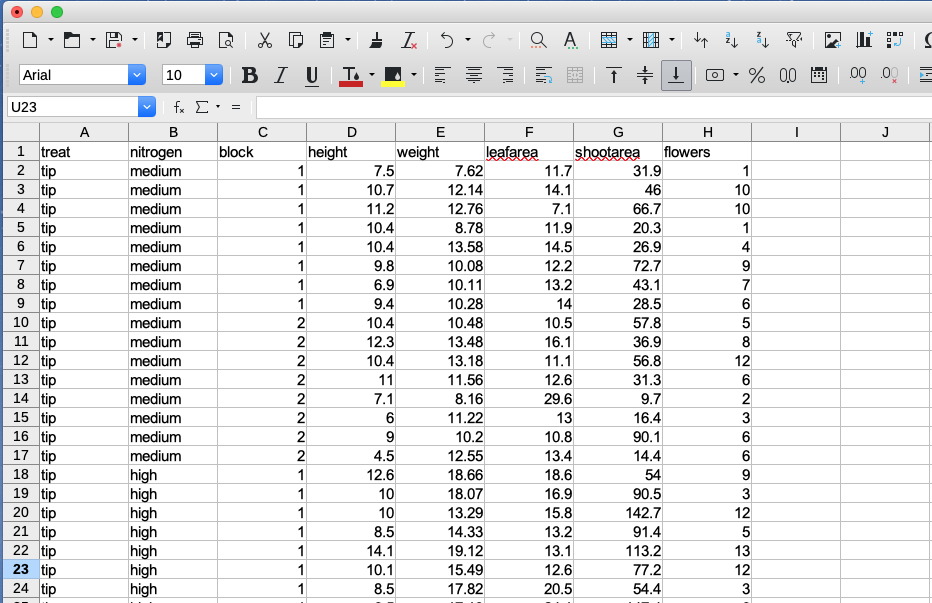
\includegraphics[width=\textwidth]{libre_off}
\colc

\vfill

\bi
\li {\bf Beware!} \url{https://genomebiology.biomedcentral.com/articles/10.1186/s13059-016-1044-7}
\ei
\end{frame}

\bfr{Importing}
\lsting{\scriptsize}
flowers <- read.table(file = 'data/flower.txt',
                      header = TRUE, sep = "\t",
                      stringsAsFactors = TRUE)
\end{lstlisting}

\bi
\li Forward slash works on ALL systems.
\li \verb|header=TRUE| means the first line is variable names.
\li \verb|sep="\t"| for tab-delimited files
\li \verb|sep=","| for comma-delimited files
\ei
\end{frame}


\bfr{Importing}
\lsting{\tiny}
> str(flowers) 
'data.frame':    96 obs. of  8 variables:
  $ treat    : Factor w/ 2 levels "notip","tip": 2 2 2 2 2 2 2 2 2 2 ...
  $ nitrogen : Factor w/ 3 levels "high","low","medium": 3 3 3 3 3 3 3 3 3 3 ...
  $ block    : int  1 1 1 1 1 1 1 1 2 2 ...
  $ height   : num  7.5 10.7 11.2 10.4 10.4 9.8 6.9 9.4 10.4 12.3 ...
  $ weight   : num  7.62 12.14 12.76 8.78 13.58 ...
  $ leafarea : num  11.7 14.1 7.1 11.9 14.5 12.2 13.2 14 10.5 16.1 ...
  $ shootarea: num  31.9 46 66.7 20.3 26.9 72.7 43.1 28.5 57.8 36.9 ...
  $ flowers  : int  1 10 10 1 4 9 7 6 5 8 .
\end{lstlisting}

\bi
\li After importing check structure of data frame.
\li treat and nitrogen have been converted to factors.
\li Usually very helpful to include this as a comment block in your script.
\ei
\end{frame}

\bfr{Specialized import functions}
\lsting{\scriptsize}
# import .csv file with sep = "\t" and header = FALSE
flowers <- read.table(file = 'data/flower.txt') 

# import .csv file with sep = "," 
# and header = TRUE
flowers <- read.csv(file = 'data/flower.csv') 

# import .csv file with dec = "," and sep = ";" 
# and header = TRUE
flowers <- read.csv2(file = 'data/flower.csv') 

# import tab delim file with sep = "\t" and header = TRUE
flowers <- read.delim(file = 'data/flower.txt') 
\end{lstlisting}

\bi
\li Avoid importing from spreadsheet files (\verb|.xls| {\em etc.}).
\ei
\end{frame}


\bfr{Import problems}
\lsting{\scriptsize}
Error in file(file, "rt") : cannot open the connection
In addition: Warning message:
In file(file, "rt") :
  cannot open file 'flower.txt': No such file or directory
\end{lstlisting}
\bi
\li Spelling mistakes.
\li Wrong working directory.
\li Forgot the extension (\verb|.txt|, \verb|.csv|, {\em etc.}).
\ei
\end{frame}

\bfr{Forgot {\tt header = TRUE}}
\lsting{\scriptsize}
flowers_bad <- read.table(file = 'data/flower.txt',
                          sep = "\t")
str(flowers_bad)
## 'data.frame':    97 obs. of  8 variables:
##  $ V1: chr  "treat" "tip" "tip" "tip" ...
##  $ V2: chr  "nitrogen" "medium" "medium" "medium" ...
##  $ V3: chr  "block" "1" "1" "1" ...
##  $ V4: chr  "height" "7.5" "10.7" "11.2" ...
##  $ V5: chr  "weight" "7.62" "12.14" "12.76" ...
##  $ V6: chr  "leafarea" "11.7" "14.1" "7.1" ...
##  $ V7: chr  "shootarea" "31.9" "46" "66.7" ...
##  $ V8: chr  "flowers" "1" "10" "10" ...
\end{lstlisting}
\bi
\li All of our variables are character (or factor).
\li The first value of each variable is the column name.
\li R has provided default names, \verb|V1, V2, V3, ...|
\ei
\end{frame}

\bfr{Alternative loader functions}
\lsting{\scriptsize}
library(readr)
# import white space delimited files
all_data <- read_table(file = 'data/flower.txt',
                       col_names = TRUE)

# import comma delimited files
all_data <- read_csv(file = 'data/flower.txt')

# import tab delimited files
all_data <- read_delim(file = 'data/flower.txt', 
                       delim = "\t")

# or use
all_data <- read_tsv(file = 'data/flower.txt')
\end{lstlisting}
\bi
\li \verb|readr| is from the {\bf tidyverse} collection of packages.
\li Many of the arguments are the same as \verb|read.table|
\li Returns a \verb|tibble|, which is very similar to a data frame.
\ei

\end{frame}

\bfr{Packages for large datasets}
\bi
\li \verb|read.table|
\li \verb|ff|
\li \verb|bigmemory|
\ei

\end{frame}


\bfr{Wrangling data frames}
\lsting{\tiny}
flowers <- read.table(file = 'data/flower.txt', header = TRUE, sep = "\t")
str(flowers)
## 'data.frame':    96 obs. of  8 variables:
##  $ treat    : chr  "tip" "tip" "tip" "tip" ...
##  $ nitrogen : chr  "medium" "medium" "medium" "medium" ...
##  $ block    : int  1 1 1 1 1 1 1 1 2 2 ...
##  $ height   : num  7.5 10.7 11.2 10.4 10.4 9.8 6.9 9.4 10.4 12.3 ...
##  $ weight   : num  7.62 12.14 12.76 8.78 13.58 ...
##  $ leafarea : num  11.7 14.1 7.1 11.9 14.5 12.2 13.2 14 10.5 16.1 ...
##  $ shootarea: num  31.9 46 66.7 20.3 26.9 72.7 43.1 28.5 57.8 36.9 ...
##  $ flowers  : int  1 10 10 1 4 9 7 6 5 8 ...
\end{lstlisting}

\end{frame}

\bfr{The \$ notation}

\lsting{\scriptsize}
flowers$height
 [1]  7.5 10.7 11.2 10.4 10.4  9.8  6.9  9.4 10.4 12.3 10.4
[12] 11.0  7.1  6.0  9.0  4.5 12.6 10.0 10.0  8.5 14.1 10.1
[23]  8.5  6.5 11.5  7.7  6.4  8.8  9.2  6.2  6.3 17.2  8.0
[34]  8.0  6.4  7.6  9.7 12.3  9.1  8.9  7.4  3.1  7.9  8.8
[45]  8.5  5.6 11.5  5.8  5.6  5.3  7.5  4.1  3.5  8.5  4.9
[56]  2.5  5.4  3.9  5.8  4.5  8.0  1.8  2.2  3.9  8.5  8.5
[67]  6.4  1.2  2.6 10.9  7.2  2.1  4.7  5.0  6.5  2.6  6.0
[78]  9.3  4.6  5.2  3.9  2.3  5.2  2.2  4.5  1.8  3.0  3.7
[89]  2.4  5.7  3.7  3.2  3.9  3.3  5.5  4.4

f_height <- flowers$height
mean(f_height)
## [1] 6.839583
summary(f_height)
##    Min. 1st Qu.  Median    Mean 3rd Qu.    Max. 
##   1.200   4.475   6.450   6.840   9.025  17.200

mean(flowers$height)
## [1] 6.839583
summary(flowers$height)
##    Min. 1st Qu.  Median    Mean 3rd Qu.    Max. 
##   1.200   4.475   6.450   6.840   9.025  17.200
\end{lstlisting}

\end{frame}

\bfr{Positional indexes}

\lsting{\scriptsize}
flowers[1, 4]
## [1] 7.5

# this would give you the same
flowers$height[1]
## [1] 7.5
\end{lstlisting}

\end{frame}

\bfr{Positional indexes}

\lsting{\scriptsize}
flowers[1:10, 1:4]
##    treat nitrogen block height
## 1    tip   medium     1    7.5
## 2    tip   medium     1   10.7
## 3    tip   medium     1   11.2
## 4    tip   medium     1   10.4
## 5    tip   medium     1   10.4
## 6    tip   medium     1    9.8
## 7    tip   medium     1    6.9
## 8    tip   medium     1    9.4
## 9    tip   medium     2   10.4
## 10   tip   medium     2   12.3
\end{lstlisting}

\end{frame}

\bfr{Positional indexes}

\lsting{\scriptsize}
flowers[c(1, 5, 12, 30), c(1, 3, 6, 8)]
##    treat block leafarea flowers
## 1    tip     1     11.7       1
## 5    tip     1     14.5       4
## 12   tip     2     12.6       6
## 30   tip     2     11.6       5
\end{lstlisting}

\end{frame}

\bfr{Empty index means "all of them"}

\lsting{\tiny}
flowers[1:8, ]
##   treat nitrogen block height weight leafarea shootarea flowers
## 1   tip   medium     1    7.5   7.62     11.7      31.9       1
## 2   tip   medium     1   10.7  12.14     14.1      46.0      10
## 3   tip   medium     1   11.2  12.76      7.1      66.7      10
## 4   tip   medium     1   10.4   8.78     11.9      20.3       1
## 5   tip   medium     1   10.4  13.58     14.5      26.9       4
## 6   tip   medium     1    9.8  10.08     12.2      72.7       9
## 7   tip   medium     1    6.9  10.11     13.2      43.1       7
## 8   tip   medium     1    9.4  10.28     14.0      28.5       6
\end{lstlisting}

\end{frame}

\bfr{Negative numbers mean "not these"}

\lsting{\scriptsize}
flowers[-(1:85), -c(4, 7, 8)]
##    treat nitrogen block weight leafarea
## 86 notip      low     1   6.01     17.6
## 87 notip      low     1   9.93     12.0
## 88 notip      low     1   7.03      7.9
## 89 notip      low     2   9.10     14.5
## 90 notip      low     2   9.05      9.6
## 91 notip      low     2   8.10     10.5
## 92 notip      low     2   7.45     14.1
## 93 notip      low     2   9.19     12.4
## 94 notip      low     2   8.92     11.6
## 95 notip      low     2   8.44     13.5
## 96 notip      low     2  10.60     16.2
\end{lstlisting}

\end{frame}

\bfr{Can also use column names}

\lsting{\scriptsize}
flowers[1:5, c("treat", "nitrogen", "leafarea")]
##   treat nitrogen leafarea
## 1   tip   medium     11.7
## 2   tip   medium     14.1
## 3   tip   medium      7.1
## 4   tip   medium     11.9
## 5   tip   medium     14.5
\end{lstlisting}

\bi
\li More readable and portable than \verb|flowers[1:5, c(1, 2, 6)]|
\ei

\end{frame}


\bfr{Logical indexes}

\lsting{\tiny}
big_flowers <- flowers[flowers$height > 12, ]
big_flowers
##    treat nitrogen block height weight leafarea shootarea flowers
## 10   tip   medium     2   12.3  13.48     16.1      36.9       8
## 17   tip     high     1   12.6  18.66     18.6      54.0       9
## 21   tip     high     1   14.1  19.12     13.1     113.2      13
## 32   tip     high     2   17.2  19.20     10.9      89.9      14
## 38   tip      low     1   12.3  11.27     13.7      28.7       5
\end{lstlisting}


\end{frame}


\bfr{Logical indexes}

\lsting{\tiny}
nit_high <- flowers[flowers$nitrogen == "high", ]        
nit_high
##    treat nitrogen block height weight leafarea shootarea flowers
## 17   tip     high     1   12.6  18.66     18.6      54.0       9
## 18   tip     high     1   10.0  18.07     16.9      90.5       3
## 19   tip     high     1   10.0  13.29     15.8     142.7      12
## 20   tip     high     1    8.5  14.33     13.2      91.4       5
## 21   tip     high     1   14.1  19.12     13.1     113.2      13
## 22   tip     high     1   10.1  15.49     12.6      77.2      12
....
\end{lstlisting}


\end{frame}


\bfr{Logical indexes}

\lsting{\tiny}
low_notip_high6 <- flowers[flowers$height >= 6 & 
                           flowers$nitrogen == "medium" &
                           flowers$treat == "notip", ]        
low_notip_high6
##    treat nitrogen block height weight leafarea shootarea flowers
## 51 notip   medium     1    7.5  13.60     13.6     122.2      11
## 54 notip   medium     1    8.5  10.04     12.3     113.6       4
## 61 notip   medium     2    8.0  11.43     12.6      43.2      14
\end{lstlisting}


\end{frame}



\bfr{Logical indexes using {\tt subset}}

\lsting{\tiny}
tip_med_2 <- subset(flowers, treat == "tip" &
                    nitrogen == "medium" & 
                    block == 2)
tip_med_2
##    treat nitrogen block height weight leafarea shootarea flowers
## 9    tip   medium     2   10.4  10.48     10.5      57.8       5
## 10   tip   medium     2   12.3  13.48     16.1      36.9       8
## 11   tip   medium     2   10.4  13.18     11.1      56.8      12
## 12   tip   medium     2   11.0  11.56     12.6      31.3       6
## 13   tip   medium     2    7.1   8.16     29.6       9.7       2
## 14   tip   medium     2    6.0  11.22     13.0      16.4       3
## 15   tip   medium     2    9.0  10.20     10.8      90.1       6
## 16   tip   medium     2    4.5  12.55     13.4      14.4       6
\end{lstlisting}
\bi
\li We don't need to use \verb|flowers$treat|
\ei

\end{frame}

\bfr{Logical indexes using {\tt subset} and {\tt select}}

\lsting{\scriptsize}
tipplants <- subset(flowers,
               treat == "tip" &  
               nitrogen == "medium" & 
               block == 2, 
               select = c("treat", "nitrogen", "leafarea"))
tipplants
##    treat nitrogen leafarea
## 9    tip   medium     10.5
## 10   tip   medium     16.1
## 11   tip   medium     11.1
## 12   tip   medium     12.6
## 13   tip   medium     29.6
## 14   tip   medium     13.0
## 15   tip   medium     10.8
## 16   tip   medium     13.4
\end{lstlisting}
\bi
\li Selecting both rows and columns.
\ei

\end{frame}

\bfr{Ordering data frames}
\lsting{\tiny}
height_ord <- flowers[order(flowers$height), ]        
height_ord
##    treat nitrogen block height weight leafarea shootarea flowers
## 68 notip     high     1    1.2  18.24     16.6     148.1       7
## 62 notip   medium     2    1.8  10.47     11.8     120.8       9
## 86 notip      low     1    1.8   6.01     17.6      46.2       4
## 72 notip     high     1    2.1  19.15     15.6     176.7       6
## 63 notip   medium     2    2.2  10.70     15.3      97.1       7
## 84 notip      low     1    2.2   9.97      9.6      63.1       2
## 82 notip      low     1    2.3   7.28     13.8      32.8       6
## 89 notip      low     2    2.4   9.10     14.5      78.7       8
## 56 notip   medium     1    2.5  14.85     17.5      77.8      10
## 69 notip     high     1    2.6  16.57     17.1     141.1       3
## 76 notip     high     2    2.6  18.88     16.4     181.5      14
## 87 notip      low     1    3.0   9.93     12.0      56.6       6
## 42   tip      low     2    3.1   8.74     16.1      39.1       3
...
\end{lstlisting}
\end{frame}


\bfr{Ordering data frames}
\lsting{\tiny}
leafarea_ord <- flowers[order(flowers$leafarea, decreasing = TRUE), ]        
leafarea_ord
##    treat nitrogen block height weight leafarea shootarea flowers
## 70 notip     high     1   10.9  17.22     49.2     189.6      17
## 13   tip   medium     2    7.1   8.16     29.6       9.7       2
## 24   tip     high     1    6.5  17.13     24.1     147.4       6
## 65 notip     high     1    8.5  22.53     20.8     166.9      16
## 23   tip     high     1    8.5  17.82     20.5      54.4       3
## 66 notip     high     1    8.5  17.33     19.8     184.4      12
## 73 notip     high     2    4.7  13.42     19.8     124.7       5
## 80 notip     high     2    5.2  17.70     19.1     181.1       8
## 17   tip     high     1   12.6  18.66     18.6      54.0       9
## 49 notip   medium     1    5.6  11.03     18.6      49.9       8
## 78 notip     high     2    9.3  18.75     18.4     181.1      16
...
\end{lstlisting}
\end{frame}



\bfr{Ordering data frames}
\lsting{\tiny}
block_height_ord <- flowers[order(flowers$block, flowers$height), ]        
block_height_ord
##    treat nitrogen block height weight leafarea shootarea flowers
## 68 notip     high     1    1.2  18.24     16.6     148.1       7
## 86 notip      low     1    1.8   6.01     17.6      46.2       4
## 72 notip     high     1    2.1  19.15     15.6     176.7       6
## 84 notip      low     1    2.2   9.97      9.6      63.1       2
## 82 notip      low     1    2.3   7.28     13.8      32.8       6
## 56 notip   medium     1    2.5  14.85     17.5      77.8      10
## 69 notip     high     1    2.6  16.57     17.1     141.1       3
....
## 38   tip      low     1   12.3  11.27     13.7      28.7       5
## 17   tip     high     1   12.6  18.66     18.6      54.0       9
## 21   tip     high     1   14.1  19.12     13.1     113.2      13
## 62 notip   medium     2    1.8  10.47     11.8     120.8       9
## 63 notip   medium     2    2.2  10.70     15.3      97.1       7
## 89 notip      low     2    2.4   9.10     14.5      78.7       8
## 76 notip     high     2    2.6  18.88     16.4     181.5      14
## 42   tip      low     2    3.1   8.74     16.1      39.1       3
## 92 notip      low     2    3.2   7.45     14.1      38.1       4
....
\end{lstlisting}
\end{frame}




\bfr{Ordering data frames}
\lsting{\tiny}
block_revheight_ord <- flowers[order(flowers$block, -flowers$height), ]        
block_revheight_ord
##    treat nitrogen block height weight leafarea shootarea flowers
## 21   tip     high     1   14.1  19.12     13.1     113.2      13
## 17   tip     high     1   12.6  18.66     18.6      54.0       9
## 38   tip      low     1   12.3  11.27     13.7      28.7       5
## 3    tip   medium     1   11.2  12.76      7.1      66.7      10
## 70 notip     high     1   10.9  17.22     49.2     189.6      17
## 2    tip   medium     1   10.7  12.14     14.1      46.0      10
## 4    tip   medium     1   10.4   8.78     11.9      20.3       1
## 5    tip   medium     1   10.4  13.58     14.5      26.9       4
## 22   tip     high     1   10.1  15.49     12.6      77.2      12
....
## 72 notip     high     1    2.1  19.15     15.6     176.7       6
## 86 notip      low     1    1.8   6.01     17.6      46.2       4
## 68 notip     high     1    1.2  18.24     16.6     148.1       7
## 32   tip     high     2   17.2  19.20     10.9      89.9      14
## 10   tip   medium     2   12.3  13.48     16.1      36.9       8
## 25   tip     high     2   11.5  23.89     14.3     101.5      12
## 47   tip      low     2   11.5   8.72     10.2      28.3       6
## 12   tip   medium     2   11.0  11.56     12.6      31.3       6
....
\end{lstlisting}
\end{frame}



\bfr{Ordering data frames}
\lsting{\tiny}
revheight_ord <- flowers[order(-xtfrm(flowers$nitrogen), flowers$height), ]        
revheight_ord
##    treat nitrogen block height weight leafarea shootarea flowers
## 62 notip   medium     2    1.8  10.47     11.8     120.8       9
## 63 notip   medium     2    2.2  10.70     15.3      97.1       7
## 56 notip   medium     1    2.5  14.85     17.5      77.8      10
## 53 notip   medium     1    3.5  12.93     16.6     109.3       3
## 58 notip   medium     2    3.9   9.07      9.6      90.4       7
## 64 notip   medium     2    3.9  12.97     17.0      97.5       5
## 52 notip   medium     1    4.1  12.58     13.9     136.6      11
....
## 2    tip   medium     1   10.7  12.14     14.1      46.0      10
## 12   tip   medium     2   11.0  11.56     12.6      31.3       6
## 3    tip   medium     1   11.2  12.76      7.1      66.7      10
## 10   tip   medium     2   12.3  13.48     16.1      36.9       8
## 86 notip      low     1    1.8   6.01     17.6      46.2       4
## 84 notip      low     1    2.2   9.97      9.6      63.1       2
## 82 notip      low     1    2.3   7.28     13.8      32.8       6
## 89 notip      low     2    2.4   9.10     14.5      78.7       8
....
## 39   tip      low     1    9.1   8.96      9.7      23.8       3
## 37   tip      low     1    9.7   6.49      8.1      18.0       3
## 47   tip      low     2   11.5   8.72     10.2      28.3       6
## 38   tip      low     1   12.3  11.27     13.7      28.7       5
## 68 notip     high     1    1.2  18.24     16.6     148.1       7
## 72 notip     high     1    2.1  19.15     15.6     176.7       6
## 69 notip     high     1    2.6  16.57     17.1     141.1       3
....
\end{lstlisting}
\end{frame}


\bfr{Ordering data frames}
\lsting{\tiny}
flowers$nitrogen <- factor(flowers$nitrogen, 
                           levels = c("low", "medium", "high"))    
nit_ord <- flowers[order(flowers$nitrogen),]
nit_ord
##    treat nitrogen block height weight leafarea shootarea flowers
## 33   tip      low     1    8.0   6.88      9.3      16.1       4
## 34   tip      low     1    8.0  10.23     11.9      88.1       4
## 35   tip      low     1    6.4   5.97      8.7       7.3       2
## 36   tip      low     1    7.6  13.05      7.2      47.2       8
## 37   tip      low     1    9.7   6.49      8.1      18.0       3
## 38   tip      low     1   12.3  11.27     13.7      28.7       5
....
## 93 notip      low     2    3.9   9.19     12.4      52.6       9
## 94 notip      low     2    3.3   8.92     11.6      55.2       6
## 95 notip      low     2    5.5   8.44     13.5      77.6       9
## 96 notip      low     2    4.4  10.60     16.2      63.3       6
## 1    tip   medium     1    7.5   7.62     11.7      31.9       1
## 2    tip   medium     1   10.7  12.14     14.1      46.0      10
## 3    tip   medium     1   11.2  12.76      7.1      66.7      10
....
## 61 notip   medium     2    8.0  11.43     12.6      43.2      14
## 62 notip   medium     2    1.8  10.47     11.8     120.8       9
## 63 notip   medium     2    2.2  10.70     15.3      97.1       7
## 64 notip   medium     2    3.9  12.97     17.0      97.5       5
## 17   tip     high     1   12.6  18.66     18.6      54.0       9
## 18   tip     high     1   10.0  18.07     16.9      90.5       3
## 19   tip     high     1   10.0  13.29     15.8     142.7      12
## 20   tip     high     1    8.5  14.33     13.2      91.4       5
....
\end{lstlisting}
\end{frame}

\bfr{Adding rows to a data frame}
\lsting{\scriptsize}
# rbind for rows
df1 <- data.frame(id = 1:4, height = c(120, 150, 132, 122),
                        weight = c(44, 56, 49, 45))
df1
##   id height weight
## 1  1    120     44
## 2  2    150     56
## 3  3    132     49
## 4  4    122     45

df2 <- data.frame(id = 5:6, height = c(119, 110),
                        weight = c(39, 35))
df2
##   id height weight
## 1  5    119     39
## 2  6    110     35
\end{lstlisting}
\end{frame}

\bfr{Adding rows to a data frame}
\lsting{\scriptsize}
df_rcomb <- rbind(df1, df2)
df_rcomb
##   id height weight
## 1  1    120     44
## 2  2    150     56
## 3  3    132     49
## 4  4    122     45
## 5  5    119     39
## 6  6    110     35
\end{lstlisting}
\end{frame}


\bfr{Adding columns to a data frame}
\lsting{\scriptsize}
df3 <- data.frame(id = 1:4, height = c(120, 150, 132, 122),
                        weight = c(44, 56, 49, 45))
df3
##   id height weight
## 1  1    120     44
## 2  2    150     56
## 3  3    132     49
## 4  4    122     45

df4 <- data.frame(location = c("UK", "CZ", "CZ", "UK"))
df4
##   location
## 1       UK
## 2       CZ
## 3       CZ
## 4       UK
\end{lstlisting}
\end{frame}


\bfr{Adding columns to a data frame}
\lsting{\scriptsize}
df_ccomb <- cbind(df3, df4)
df_ccomb
##   id height weight location
## 1  1    120     44       UK
## 2  2    150     56       CZ
## 3  3    132     49       CZ
## 4  4    122     45       UK
\end{lstlisting}
\end{frame}

\bfr{Adding computed columns to a data frame}
\lsting{\scriptsize}
df_rcomb$height_log10 <- log10(df_rcomb$height)
df_rcomb
##   id height weight height_log10
## 1  1    120     44     2.079181
## 2  2    150     56     2.176091
## 3  3    132     49     2.120574
## 4  4    122     45     2.086360
## 5  5    119     39     2.075547
## 6  6    110     35     2.041393
\end{lstlisting}
\end{frame}

\bfr{Converting type of a column}
\lsting{\tiny}
# convert to a factor 
df_rcomb$Fid <- factor(df_rcomb$id)
df_rcomb
##   id height weight height_log10 Fid
## 1  1    120     44     2.079181   1
## 2  2    150     56     2.176091   2
## 3  3    132     49     2.120574   3
## 4  4    122     45     2.086360   4
## 5  5    119     39     2.075547   5
## 6  6    110     35     2.041393   6
str(df_rcomb)
## 'data.frame':    6 obs. of  5 variables:
##  $ id          : int  1 2 3 4 5 6
##  $ height      : num  120 150 132 122 119 110
##  $ weight      : num  44 56 49 45 39 35
##  $ height_log10: num  2.08 2.18 2.12 2.09 2.08 ...
##  $ Fid         : Factor w/ 6 levels "1","2","3","4",..: 1 2 3 4 5 6
\end{lstlisting}
\end{frame}


\bfr{Merging data frames}
\bi
\li Suppose we have one data frame with information about some
common rocky shore invertebrates, called \verb|taxa|
\li And we have another data frame with infromation about where these invertebrates are usually found,
called \verb|zone|
\li Can we combine these into one data frame with all information about the invertebrates?
\ei
\end{frame}

\bfr{Merging data frames}
\lsting{\tiny}
taxa <- data.frame(
         GENUS = c("Patella", "Littorina", "Halichondria", "Semibalanus"),
         species = c("vulgata", "littoria", "panacea", "balanoides"),
         family = c("patellidae", "Littorinidae", "Halichondriidae", "Archaeobalanidae"))
taxa
##          GENUS    species           family
## 1      Patella    vulgata       patellidae
## 2    Littorina   littoria     Littorinidae
## 3 Halichondria    panacea  Halichondriidae
## 4  Semibalanus balanoides Archaeobalanidae

zone <- data.frame(
    genus = c("Laminaria", "Halichondria", "Xanthoria", "Littorina",
           "Semibalanus", "Fucus"),
    species = c("digitata", "panacea", "parietina", "littoria",  
            "balanoides", "serratus"),
    zone = c( "v_low", "low", "v_high", "low_mid", "high", "low_mid"))
zone
##          genus    species    zone
## 1    Laminaria   digitata   v_low
## 2 Halichondria    panacea     low
## 3    Xanthoria  parietina  v_high
## 4    Littorina   littoria low_mid
## 5  Semibalanus balanoides    high
## 6        Fucus   serratus low_mid
\end{lstlisting}
\end{frame}

\bfr{Merging data frames}
\lsting{\tiny}
taxa_zone <- merge(x = taxa, y = zone)
taxa_zone
##      species        GENUS           family        genus    zone
## 1 balanoides  Semibalanus Archaeobalanidae  Semibalanus    high
## 2   littoria    Littorina     Littorinidae    Littorina low_mid
## 3    panacea Halichondria  Halichondriidae Halichondria     low
\end{lstlisting}
\bi
\li Because the two data frames have a column name in common,
R assumes you want to join on that column.
\li The joined data frame has both \verb|GENUS| and \verb|genus| because
they are spelled differently.
\li The joined data frame has only those rows with information in BOTH
original data frames.
\ei
\end{frame}


\bfr{Merging data frames}
\lsting{\tiny}
taxa_zone <- merge(x = taxa, y = zone, all = TRUE)
taxa_zone
##      species        GENUS           family        genus    zone
## 1 balanoides  Semibalanus Archaeobalanidae  Semibalanus    high
## 2   digitata         <NA>             <NA>    Laminaria   v_low
## 3   littoria    Littorina     Littorinidae    Littorina low_mid
## 4    panacea Halichondria  Halichondriidae Halichondria     low
## 5  parietina         <NA>             <NA>    Xanthoria  v_high
## 6   serratus         <NA>             <NA>        Fucus low_mid
## 7    vulgata      Patella       patellidae         <NA>    <NA>
\end{lstlisting}
\bi
\li To include ALL data from BOTH frames use \verb|all = TRUE|
\li NAs will be substituted for missing data.
\ei
\end{frame}



\bfr{Merging data frames}
\bi
\li Use \verb|by.x| and \verb|by.y| if the names are different
\ei
\lsting{\tiny}
taxa_zone <- merge(x = taxa, y = zone, 
                   by.x = "GENUS", 
                   by.y = "genus",
                   all = TRUE)
taxa_zone
##          GENUS  species.x           family  species.y    zone
## 1        Fucus       <NA>             <NA>   serratus low_mid
## 2 Halichondria    panacea  Halichondriidae    panacea     low
## 3    Laminaria       <NA>             <NA>   digitata   v_low
## 4    Littorina   littoria     Littorinidae   littoria low_mid
## 5      Patella    vulgata       patellidae       <NA>    <NA>
## 6  Semibalanus balanoides Archaeobalanidae balanoides    high
## 7    Xanthoria       <NA>             <NA>  parietina  v_high
\end{lstlisting}

\end{frame}

\bfr{Merging data frames}
\bi
\li Can use multiple columns
\ei
\lsting{\tiny}
taxa_zone <- merge(x = taxa, y = zone, 
                   by.x = c("species", "GENUS"), 
                   by.y = c("species", "genus"), 
                   all = TRUE)
taxa_zone
##      species        GENUS           family    zone
## 1 balanoides  Semibalanus Archaeobalanidae    high
## 2   digitata    Laminaria             <NA>   v_low
## 3   littoria    Littorina     Littorinidae low_mid
## 4    panacea Halichondria  Halichondriidae     low
## 5  parietina    Xanthoria             <NA>  v_high
## 6   serratus        Fucus             <NA> low_mid
## 7    vulgata      Patella       patellidae    <NA>
\end{lstlisting}

\end{frame}





\end{document}
